The variable R studies are based on standard model VH production Monte Carlo which is discussed in section \ref{decay}. The optimisation studies are for VH resonances and is motivated in section \ref{resonance}.  
\section{Introduction}
An introduction to the process of Monte Carlo simulation and the ATLAS detector is needed before any description of the search can be understood.
\subsection{Simulation}
\label{section:Simulation}
Monte Carlo simulations are an important aspect to any analysis. Not only do they allow for refinement of analysis techniques but must also be used to compare theoretical expectation with reality.   

Simulation can be split into two parts, event generation and detector response. These two parts come sequentially with the final result compared to data as shown in figure \ref{fig:decays}. 

\begin{figure}[H]
\centering
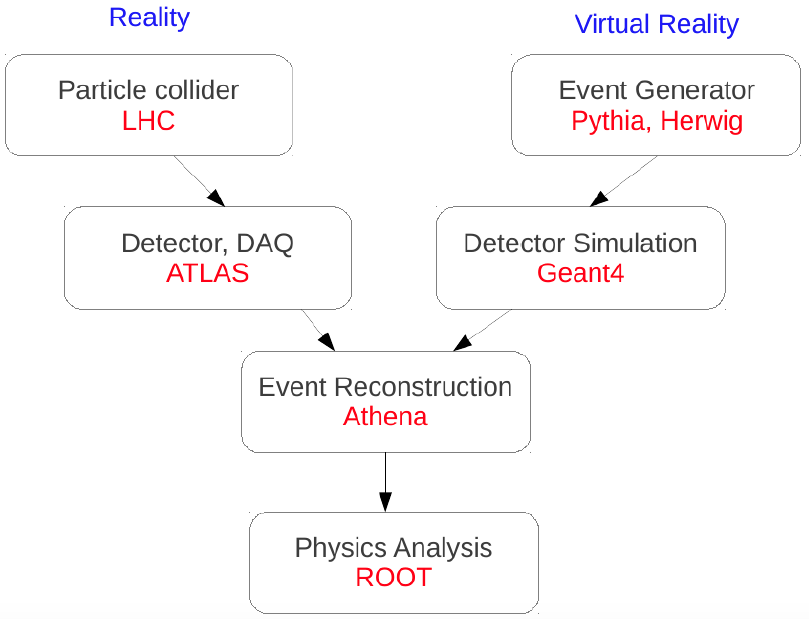
\includegraphics[scale=0.3]{figures/MC-diagram.png}
\caption{Work flow of standard analysis. \copyright John Morris.}
\label{fig:decays}
\end{figure}

The process of Monte Carlo simulation from matrix elements to our observed decays before simulation of the detector can be described approximately with 5 steps\cite{Jmorris}. These steps are shown on figure \ref{fig:guide}, and use a range of generators and models to arrive at the final state particles this analysis is interested in. The idiosyncrasy of each part are numerous, however the uncertainties associated can be briefly highlighted since they limit the accuracy of our search.
\begin{figure}[H]
\hspace{-1cm}
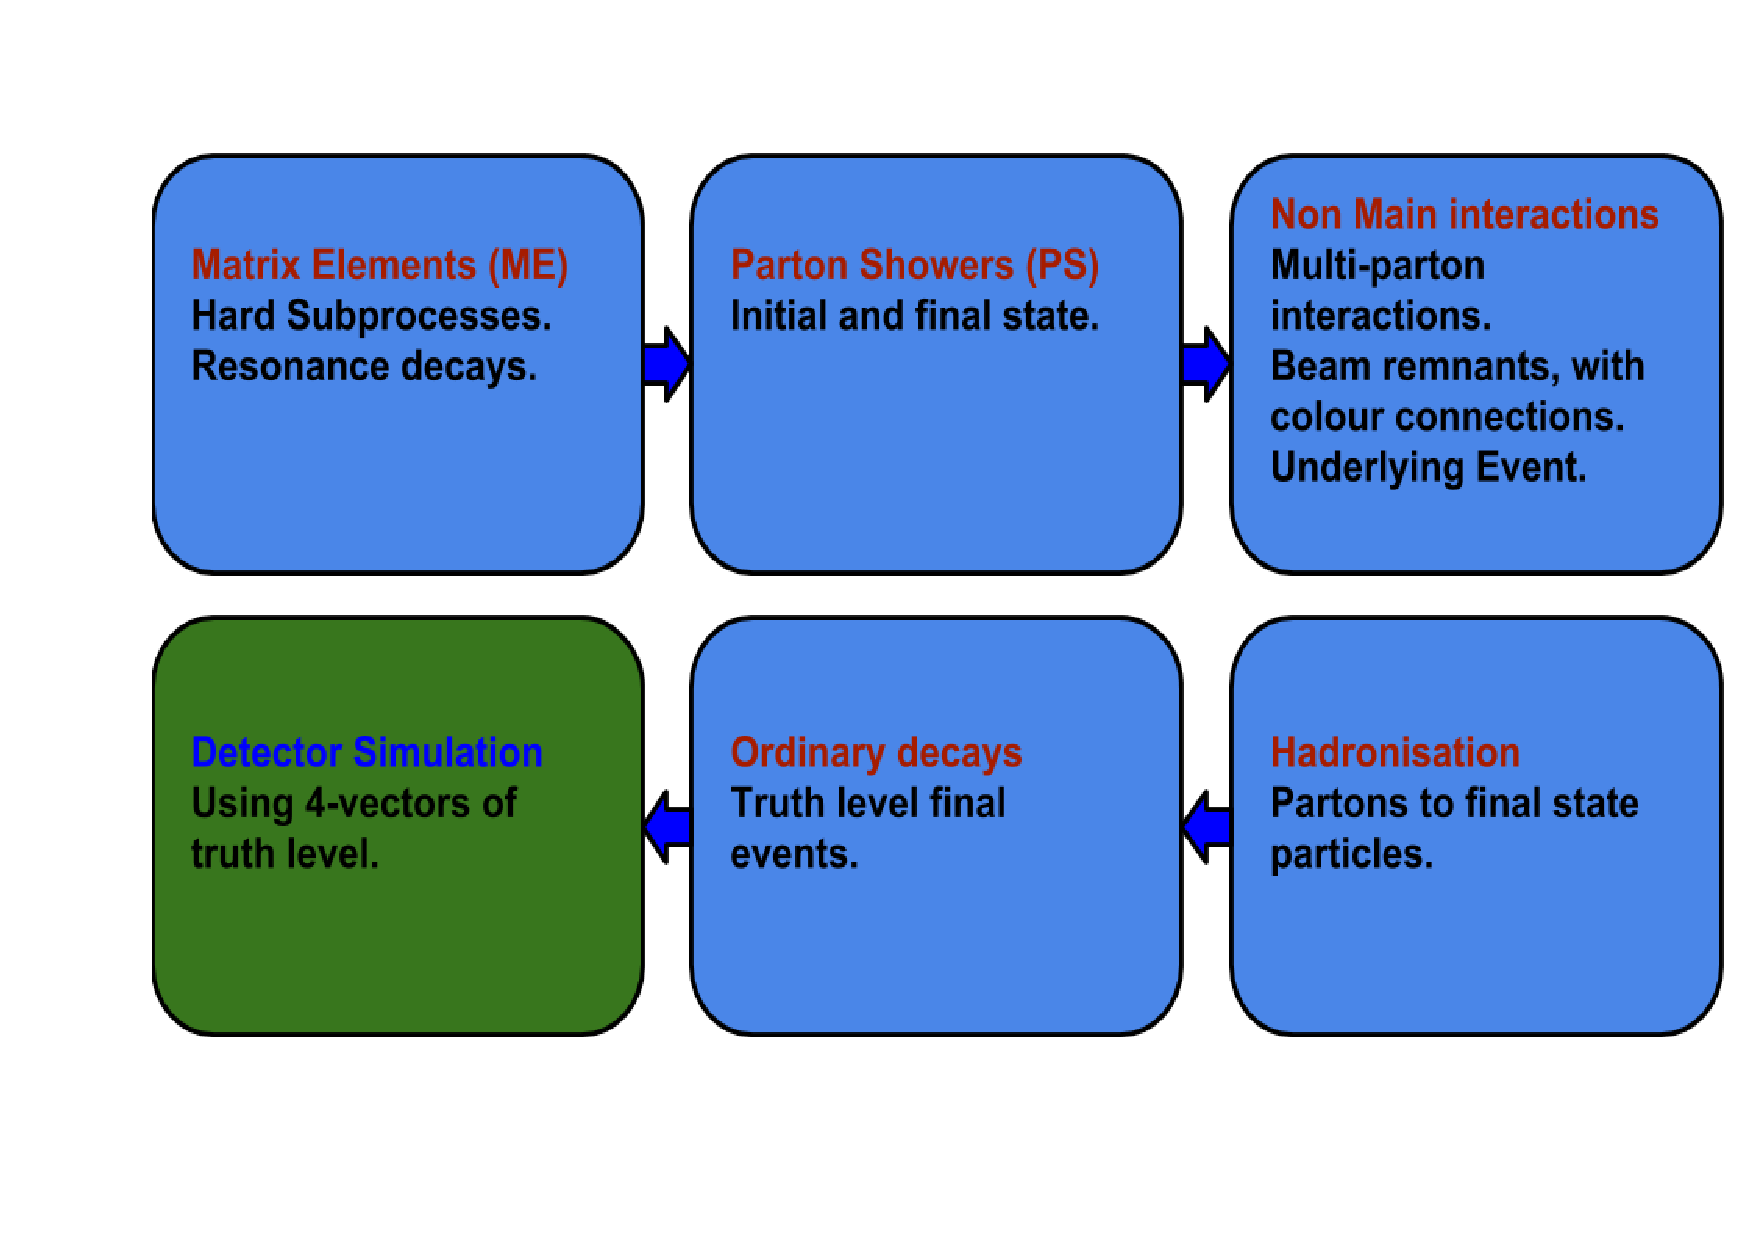
\includegraphics[scale=0.5]{figures/MC-simulation-truthEvent.pdf}
\caption{Rough guide from interaction to truth level particles. The use of the 4-vector truth information in detector simulation will also have many parts.}
\label{fig:guide}
\end{figure}

The very fact that each part can be calculated in a different way leads to theoretical modelling uncertainties. These uncertainties include generator (matrix element calculations), parton density function (PDF), parton shower (PS) and hadronization uncertainties. 
Generator uncertainties come from the limit on the order in the calculation of the matrix elements. PDF uncertainties come from the use of different parameterisations. At the LHC CTEQ, MSTW and NNPDF are used, each arriving at a different result. PS uncertainties come from the divergencies that must be avoided in any QCD calculation. How this is dealt with depends on the generator. Two common examples would come from the generators PYTHIA and HERWIG, which calculate the parton with the highest $p_T$ and angle respectively. Hadronization occurs at very low energy scales in which perturbation theory is not valid. Therefore a suitable model is needed and two approaches are often used: the Lund string and Cluster models. Each model similarly to PS modelling will produce a different result, therefore this leads to further uncertainties in the overall modelling. 

A general practice to determine the total uncertainty is by simply using different models for each calculation and taking the difference, known as the offset method. 

At this stage, known as the truth level, the simulation has produced stable final state particles with 4-vector information and all parent-daughter relations, such as b-tagging from parton level. Now the interaction of the final state particle and the detector must be considered.       
GEANT4 is used to take the output 4-vectors of the truth level generators and model the detector response. This is a very complex process and involves modelling all subdetectors of the ATLAS experiment. This modelling can be done to different degrees of accuracy to save computation time with the final output matching the output of the ATLAS detector. 
 
\subsection{The ATLAS Detector}
\label{atlasdetector}
The ATLAS detector is one of the experiments situated at an interaction point round the LHC at CERN.


The standard geometry of the ATLAS detector is a right hand coordinate system with the origin at the intersection point, the z-axis pointing along the beam pipe, the x-axis point towards the LHC centre and the y-axis to the heavens. It's natural to use the cylindrical coordinate system in many situations: this is defined with the axis of rotation round the z-axis ($\phi$) and from the z-axis ($\eta=-\ln\tan (\frac{\theta}{2}$)). The definition of $\eta$ is due to it's use to define a Lorentz invariant measure of angular separation: $R_{ij}=\sqrt{\Delta\eta_{ij} + \Delta\phi_{ij}}$.

    
The experiment can be split into three main subsystems: the inner tracker, the calorimeters and muon spectrometer\cite{atlas}. The inner tracker is composed of pixel sensors closes to the beam line and strip sensors thereafter. The whole tracker is immersed in a 2T magnetic field used to measure the momentum of charged particle from the curvature. This inner detector makes accurate measurements of position and momentum, up to $\eta < 2.5 $, and a transition radiation tracker (TRT) is situated after the silicon detector, up to a  $\eta < 2.0$. The pixel detector is essential in b-tagging using extended secondary vertices (SV) from the primary vertex (PV). The TRT is particular useful for electron identification and determination if photons are converted or not.      

The calorimeters are located beyond the solenoid and cover the range $|\eta| < 4.9 $. With a plethora of detector technologies used, the liquid argon electromagnetic (EM) calorimeters are divided into 3 sections - the barrel, endcap and forward sections - $|\eta| < 1.475 $, $1.375 < |\eta| < 3.2 $  and $3.1 < |\eta| < 4.9$. 
The hadronic calorimeters surround the EM calorimeter with a coverage of $|\eta| < 4.9$ and use a combination of scintillating tiles and liquid argon as active materials. The muon chamber uses three large air core toroidal magnets, each containing eight superconducting coils to deflect muons, to measure the curvature of the resulting track \cite{muoncham}. 

The mammoth task of reducing the 40 MHz bunch crossing rate to a manageable 300 Hz is dealt with in three stages\cite{trigger}. The first (Level 1) is hardware based and takes input mostly from muon and calorimeter trigger systems. This trigger reduces the rate to less than 75 kHz which is reduced further to $\approx$300 Hz by the next two trigger systems. These are software based on the ATLAS offline Athena framework. 



\section{The Standard Model $VH\rightarrow b\bar{b} + ll/l\nu/\nu\nu$ Decay Channel }
\label{decay}
The channel $H\rightarrow b\bar{b}$ is particularly difficulty to detect due to the large MultiJet (MJ) background at the LHC. Combined with other backgrounds this makes the most prominent decay channel invisible. The association of a vector boson gives a clear signature in the muon and calorimeter trigger systems which allows the identification of the Higgs over many backgrounds.  

The focus on the VH production to tag the $H\rightarrow b\bar{b}$ decay will remove some but not all backgrounds. Different types of background decays will pollute the signal yield to different extents. The more similar the decay products of the background to the signal, the more difficult to differentiate. 
The main backgrounds come from (W/Z)+jets and $t\bar{t}$ production with smaller contributions made from single top, diboson production (WW,WZ,ZZ)  and MJ \cite{higgsBB}. Top quarks decay over 99\% of the time via $t\rightarrow W b$. With a combination of leptons, neutrinos and actual b-tagged jets for each top decay, this process can be easily confused for signal. The same is true with (W/Z) + jets and diboson production, i.e the final state is similar to the signal final state. The MJ background refers to any event with multiple jets but no prompt isolated electrons or muons \cite{multijetsusy}. This background comes in two forms. One is from large energy fluctuations from jets which acts as $E_T^{miss}$ in the calorimeters and the other as misidentified electrons. The first pollutes the signal in the 0 lepton channel and the other, both lepton channels.

To remove these backgrounds discriminating variables must be used. The invariant mass of the dijet system would be one example. This is the invariant mass of the $b\bar{b}$ pair and must equate the Higgs mass $m_{H}$ (Note this would be defined in terms of a clustered fat jet) . If this is different from the Higgs mass then this signifies that the event was background. In the same light other internal and distributive characteristics of the jets can be used. One such substructure variable $\sqrt{d12}$ - which is the kt-splitting scale - is explained in section \ref{Significance}. 

Reliant b-tagging is another important factor for better discriminating power. This is made more difficult at high $P_T$ as the b-jets produced will become merged (unresolved). This is due to the combined momentum of the decay products having to be focused more in one direction. The geometric matching between the truth B-hadron and reconstructed jet is crucial for high b-tagging efficiency. The performance of a new generic sequential recombination algorithm, known as the variable R jet algorithm, is employed to minimize the deltaR (The angular separation) between the B-hadron and the jet.

\subsection{Variable R Jets}
\label{VarR}
Calorimeter jets are localised clusters in the EM and Hadronic Calorimeters. Track jets are clustered tracks produced in the inner tracker. The most common clustering algorithms used are sequential recombination algorithms, which are best suited to deal with the large QCD background from the $pp$ collisions.


 The algorithms use two metrics defined in equations \ref{eq:metric}. The $p^{2n}_{Ti}$ terms correspond to the tangential momentum, with each algorithm applying their own (n) parameter which is set to $n=-1$ for the anti-$k_t$ algorithm. The $R_0$ parameter is a set constant for the full clustering process and plays a role in the jet's size. The $\Delta R_{ij}$ parameter is defined in section \ref{atlasdetector} and is between clusters in the tracker or calorimeter.
\begin{equation}
\displaystyle
d_{ij} = min(p_{Ti}^{2n},p_{Tj}^{2n})\Delta R_{ij}  \qquad  with \qquad d_{iB} = p_{Ti}^{2n}R_0 
\label{eq:metric}
\end{equation}

A summary of how each algorithm works is as follows: Using their preset value of (R) and (n); compute $d_{ij}$ and $d_{iB}$; if $d_{ij}$ is the largest then combine jets and repeat; otherwise the jet object (i) is removed as a final jet. This is repeated until the termination point set for each algorithm.

The fixed R parameter throughout the clustering process can be problematic for highly boosted decay products since the jets produced are often merged. This can be mitigated using a clustering parameter R which varies in size with jet momentum \cite{varR}.         
\begin{equation}
\displaystyle
R_{0}= R_{eff}(P_{T})=\frac{\rho}{P_{Ti}}
\label{eq:varREquation}
\end{equation}

The variable-R algorithm does this with the parameters defined in equation \ref{eq:varREquation}.

\subsection{My contribution}
The highly boosted decay products of the Higgs will often be unresolved. Therefore, the use of variable-R jets is ideal to resolve the deposited energy from the $b\bar{b}$ decay products. A comparison between the anti-$k_t$ and variable-R algorithm for different input parameters is made. Presented here is the algorithms performance at reconstructing the jet in the same direction as the truth level B-hadron. The signal sample is simulated standard model WH events decaying via $VH \rightarrow b\bar{b} + l \nu $. Figures \ref{fig:drtogether} show the geometric displacement between the reconstructed jet and the truth B-hadron.   
\begin{figure}[H]
%\centering
\hspace{-2.5cm}
\subfloat{\label{fig:drmean} 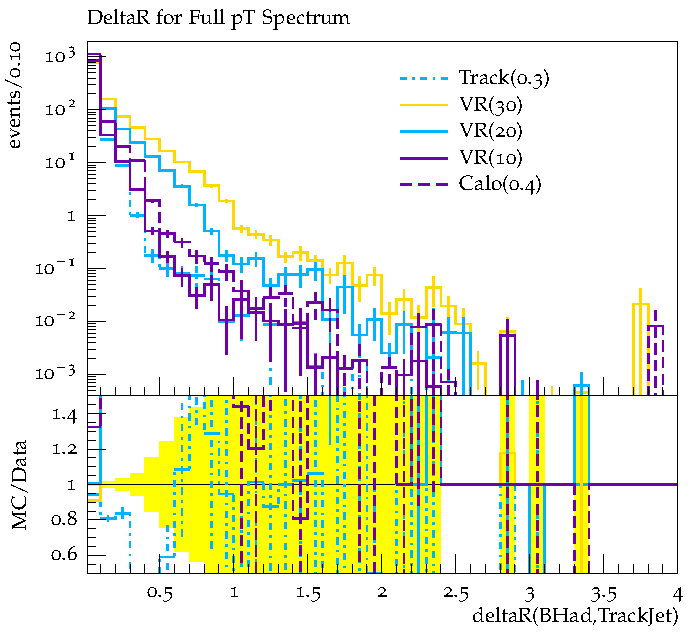
\includegraphics[width=0.65\linewidth]{figures/dr-mean-all-pT-GA-Log.pdf}}
\subfloat{\label{fig:drpt} 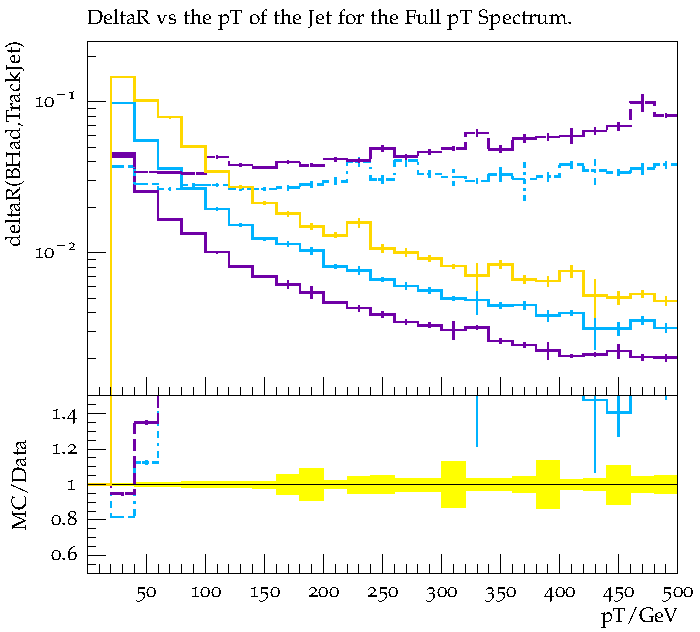
\includegraphics[width=0.65\linewidth]{figures/dr-ptJet-Full-pT-GA-Log.pdf}}
\caption{The variable deltaR(BHad,Trackjet) is the angular distance. Figure \ref{fig:drmean} illustrates how well each algorithm with different input variables matches the direction of the B-hadron. Figure \ref{fig:drpt} shows this performance over the inclusive $P_T$ of the reconstructed jet.}
\label{fig:drtogether}
\end{figure}

The variable R jet have a smaller angular displacement compared to the B-hadron. Figure \ref{fig:drpt} shows the variable-R jets with a smaller angular separation at higher $P_T$ compared to the anti-kt algorithm. 

\section{Beyond the Standard Model and $VH\rightarrow b\bar{b}$+$ll/l\nu/\nu\nu/qq$}
\label{resonance}
With the discovery of a Higgs consistent with the Standard Model the question of naturalness is under reexamination\cite{natural}. The naturalness problem arises through the corrections the Higgs mass receives from virtual particles. If the virtual particles can take any momentum to the Planck mass scale then the correction must be huge. This is strange since the Higgs mass is a relatively small, therefore it is natural to think that there must exist a cut off for the maximum momentum taken by the virtual particles.  
 The unnaturalness of the standard model motivates many theories to be put forward. Some of these dynamical electroweak symmetry breaking scenarios predict resonances which decay to a Higgs and vector boson \cite{resonance}. These will subsequently decay into many different final states, a subsection being $VH\rightarrow b\bar{b}$+$ll/l\nu/\nu\nu/qq$.

\subsection{Cut Optimisation and Significance}
\label{Significance}
The setting of exclusion limits and the determination of signal strength needs the removal of the background events and as small as possible uncertainty.
The removal of background can be done in many different ways. However a simple yet effective way is to perform a series of window cuts on a set of discriminating variables.  
This is done using the toolkit for multivariate analysis (TMVA), which is a ROOT integrated environment for the application of multivariate classification \cite{tmva}.
TMVA will maximise the background rejection for a given signal efficiency and produce the cuts corresponding to these values.

Total background rejection is not precisely what is of most interest to this search. Since this does not take into account the relative shapes of signal to background \cite{statphysics}. To shed some light on this the significance must be calculated. The calculation will show larger significance if the signal shape is drastically different from the background. The definition of significance varies from analysis to analysis. This is due to different approximations and assumptions being used. 


\subsection{My contribution}
Monte Carlo VH 1.0/1.5 TeV resonance events from the HVT model and backgrounds (W+jets, $t\bar{t}$, Z+jets and single top) with preselection cuts:
\begin{itemize}
  \item 1 lepton with pt $>$ 25 GeV;
  \item $E_{t}^{miss}$ $>$ 20 GeV; 
  \item One R=1.0 trimmed anti-kt jet with $p_t$ $>$ 250 GeV;
	\item Two b tagged 0.3 track jets ghost associated (GA) to leading large-R jet;
	\item Zero b-tagged 0.3 track jets not GA to leading large-R jet;
	\item B-tagging: Truth labeled b,c and light jets with 75\%, 10\% and 3\% tagging efficiencies respectively;
\end{itemize}
are used as input to the TMVA. The b-efficiencies are not optimal and could see further improvements. 

One topological and two substructure parameters are presented here as the discriminating variables of interest:

\begin{equation}
\displaystyle
\frac{ VH_{pt}}{H_{pt}+V_{pt}} \qquad \sqrt{d12} \qquad m_{H} 
\label{eq:discrimVar}
\end{equation}

The substructure variables $m_{H}/\sqrt{d12}$ are from the R=1.0 anti-$k_t$ jet. The splitting scale ($\sqrt{d_{12}}$) is defined as the minimum $d_{ij}$/$d_{iB}$ before the final clustering step\cite{d12}. The topological cut was found to be a powerful discriminating characteristic between signal and background for both resonance masses. This can be seen on figures \ref{fig:roc} were each variable was optimised individually. Therefore this variable is used to produce significance plots in combination with the other variables to search for any improvements.    

\begin{figure}[H]
%\centering
\hspace{-2.5cm}
\subfloat{\label{fig:roc1} 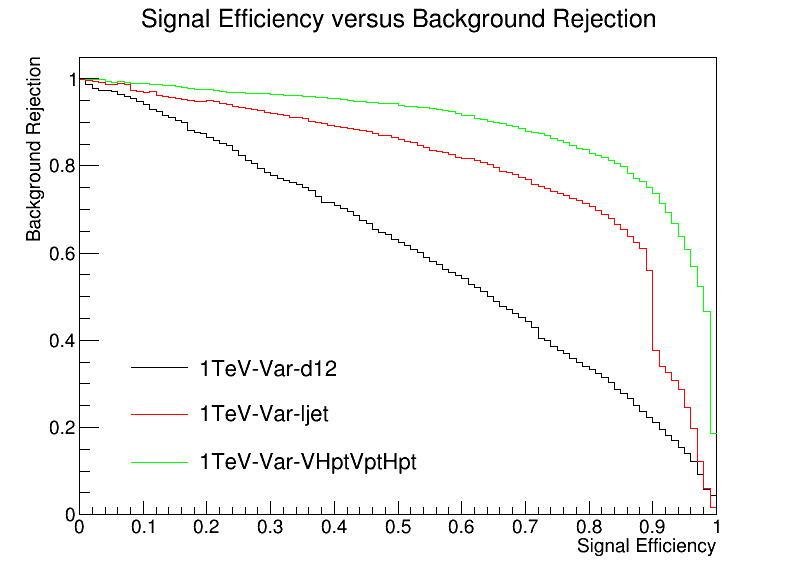
\includegraphics[width=0.65\linewidth]{figures/config-1T-Trained-alone-mass-VHScal-d12.png}}
\subfloat{\label{fig:roc1.5} 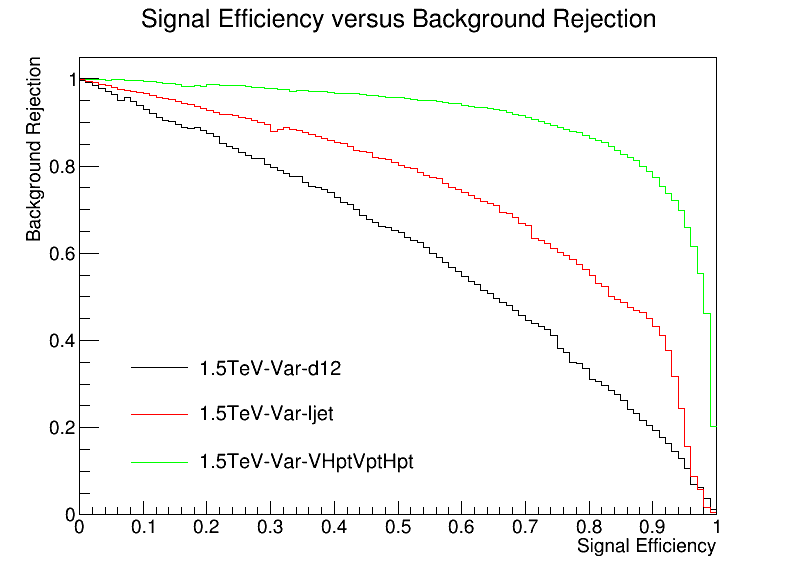
\includegraphics[width=0.65\linewidth]{figures/config-15T-Trained-alone-mass-VHScal-d12.png}}
\caption{Figure \ref{fig:roc1} shows the background rejection for a given signal efficiency for each cut trained on the 1 TeV resonance sample. Figure \ref{fig:roc1.5} shows the same thing trained on a 1.5 TeV resonance.
\textcolor{black}{Black}: $\sqrt{d12}$
\textcolor{red}{Red}: $m_{H}$
\textcolor{green}{Green}: $\frac{VH_{pt}}{H_{pt}+V_{pt}}$
}
\label{fig:roc}
\end{figure}

The behaviour of the TMVA must be checked to ensure the validity of the results. One simple way of doing this is checking the cuts the TMVA predicts to ensure they appear realistic. Figures \ref{fig:cutsVH}/\ref{fig:cuts} show the cuts for each efficiency for the ROC curves \ref{fig:roc}. The Higgs mass appears lower than 125 GeV due to the miscalibration of the jets. 

\begin{figure}[H]
\hspace{-1cm}
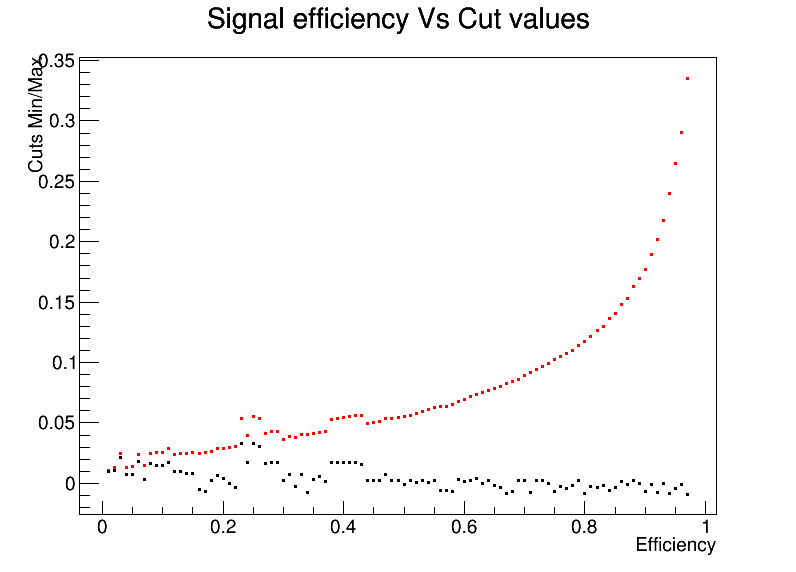
\includegraphics[scale=0.5]{figures/Cuts-VHptVptHpt.png}
\caption{The window cut on the topological variable for each efficiency. The cuts window increases from left to right due to a need for greater signal efficiency.}
\label{fig:cutsVH}
\end{figure}


\begin{figure}[H]
%\centering
\hspace{-2.5cm}
\subfloat{\label{fig:mass} 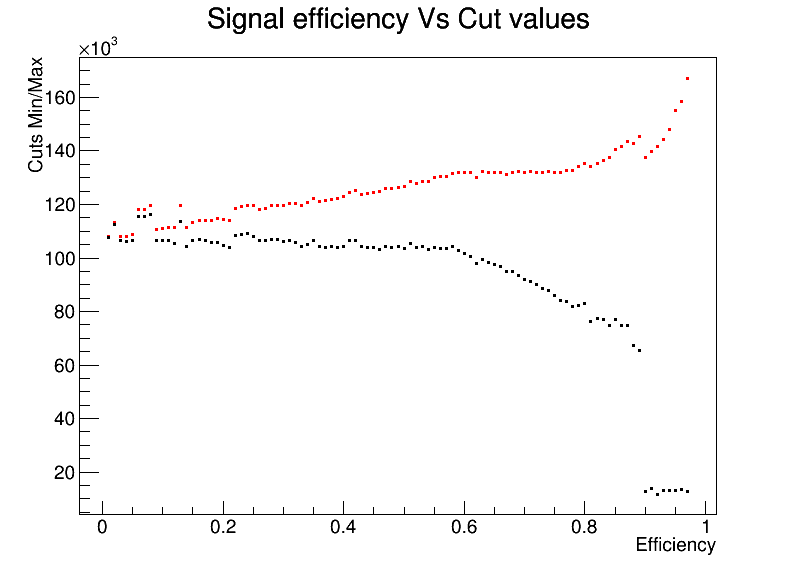
\includegraphics[width=0.65\linewidth]{figures/Cuts-ljet.png}}
\subfloat{\label{fig:d12} 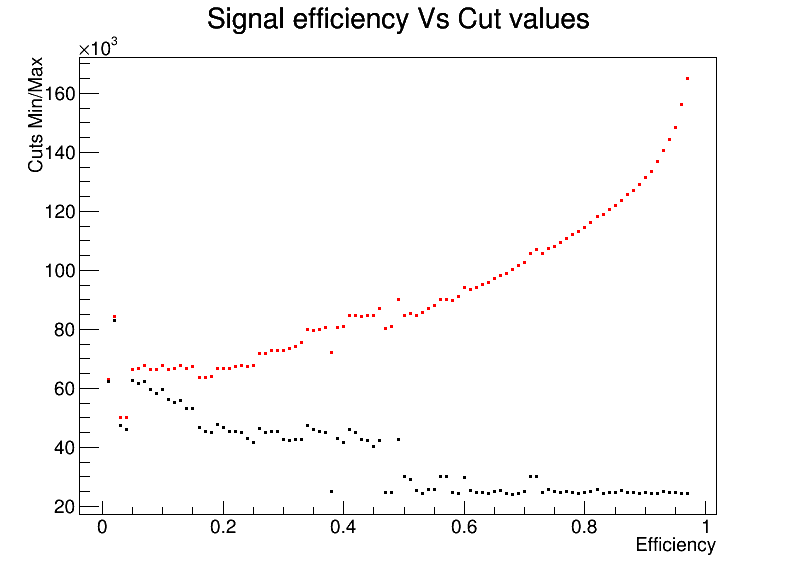
\includegraphics[width=0.65\linewidth]{figures/Cuts-d12-alone.png}}
\caption{ Figure \ref{fig:mass} shows the cuts for $m_{H}$. Figure \ref{fig:d12} shows the cuts for $\sqrt{d12}$.  }
\label{fig:cuts}
\end{figure}


The significance used is defined as as the quadrature sum of $\frac{S}{\sqrt{B}}$ per bin. This definition might not be sufficient due to the small number of signal events which is discussed in section \ref{chp:furtherwork}. The significance is calculated over the VH mass spectrum using the cuts for a particular signal efficiency.  

\begin{figure}[H]
\hspace{-1cm}
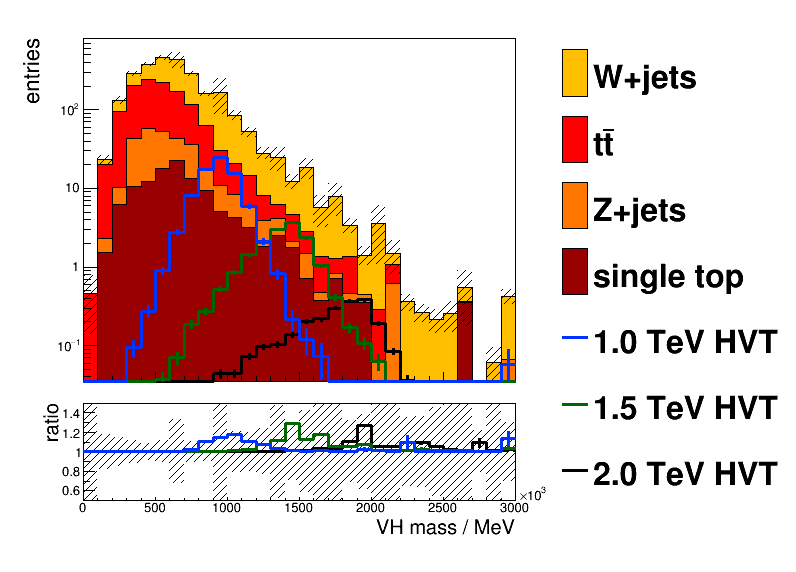
\includegraphics[scale=0.5]{figures/vh_m_log.png}
\caption{The VH mass spectrum with the resonances and backgrounds after preselection.}
\label{fig:vhspectrum}
\end{figure}

The search would like to have common selection for the 1 and 1.5 TeV resonances. Therefore only the 1.5 TeV resonance sample is used to train the TMVA and produce the necessary cuts. The cuts for the 1.5 TeV resonance were then used with the 1 TeV sample to separate signal from background and the results are shown on figures \ref{fig:vhsig}/\ref{fig:sig}.     
\begin{figure}[H]
\hspace{-1cm}
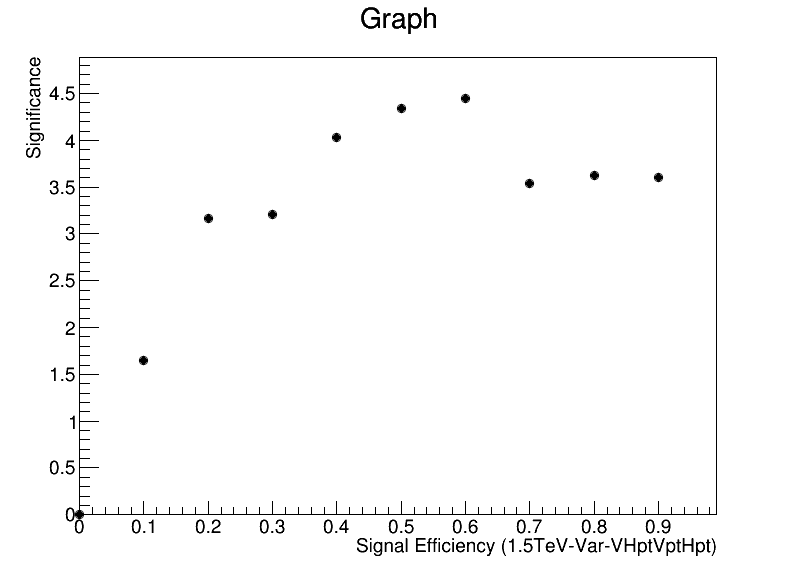
\includegraphics[scale=0.5]{figures/15TeVTrained-data10-Var-VHptVptHpt.png}
\caption{The trained TMVA cuts for 1.5 TeV used with the 1 TeV sample for the topological variable alone. }
\label{fig:vhsig}
\end{figure}


\begin{figure}[H]
%\centering
\hspace{-2.5cm}
\subfloat{\label{fig:masssig} 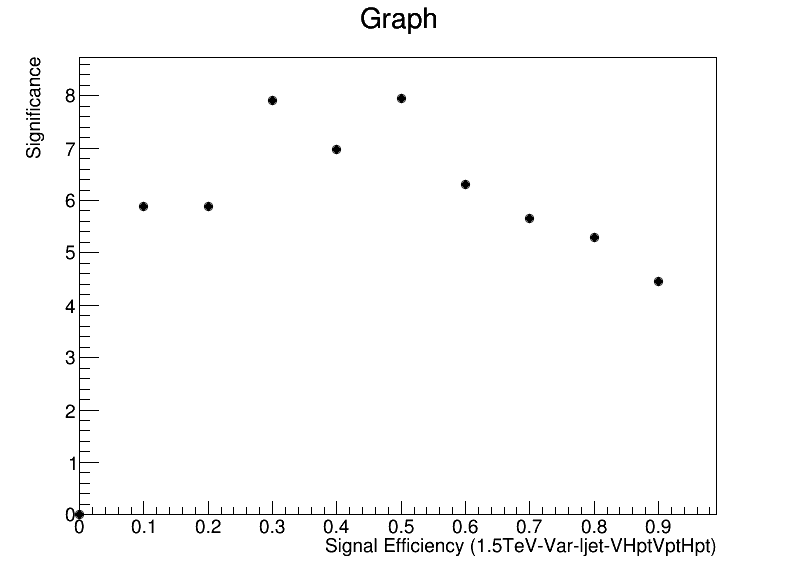
\includegraphics[width=0.65\linewidth]{figures/15TeVTrained-data10-Var-ljet-VHptVptHpt.png}}
\subfloat{\label{fig:d12sig} 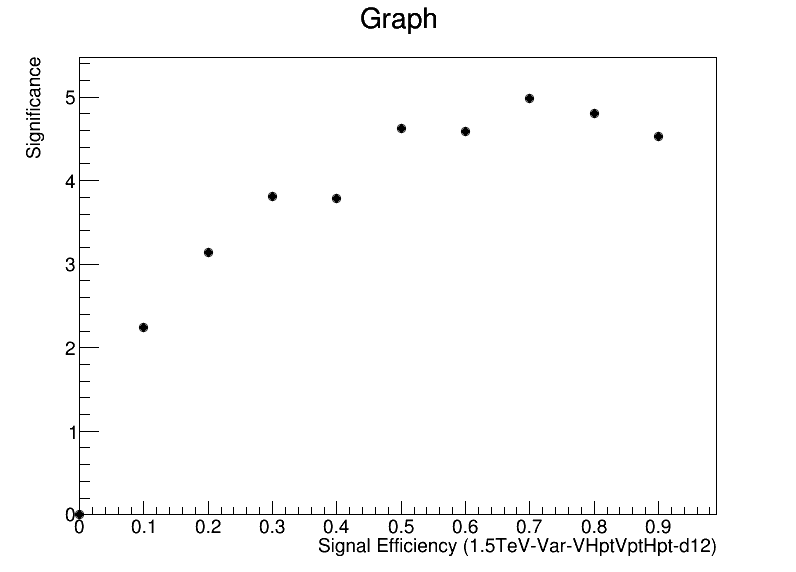
\includegraphics[width=0.65\linewidth]{figures/15TeVTrained-data10-Var-VHptVptHpt-d12.png}}
\caption{The trained TMVA cuts for 1.5 TeV used with the 1 TeV sample for the topological cut combined with $m_{b\bar{b}}$ \ref{fig:masssig} and $\sqrt{d12}$ \ref{fig:d12sig}}
\label{fig:sig}
\end{figure}

The substructure variables both have an improvement on the significance compared to the topological cut alone. The $m_{H}$ variable has the most drastic improvement. However the $\sqrt{d12}$ could seen further improvement after trimming. 
